\chapter{概览}
\label{cap:overview}
    我们模型的主要目标,就是拿到神经网络的结构,预测该神经网络在特定硬件环境下的运行时间。特别地,我们的模型针对tensorflow框架,也就是说,所有性能数据全部来源于tensorflow,因此,我们的预测结果在其他深度学习框架中不一定能够得到较好的预测结果。另一方面,我们模型主要针对CNN进行设计,能够在现有的广泛使用的CNN网络上有比较好的预测结果,如AlexNet\cite{alexnet}等。
    
\section{模型配置}
    模型的输入部分包括网络的结构或网络对应的数据流图、各个计算模块的参数、运行的硬件平台,共三部分。
    
    网络结构在执行过程中,会先转换为数据流图的形式,这一部分对深度神经网络进行主要的定义。而由于数据流图对输入的形状、维度等没有严格的限制,如图\ref{fig:dag_same}所示。因此,输入部分需要对输入的形状进行预先的定义,以便于之后模型进行模拟调度以及性能预测。
    
    另外,输入需要提供运行的硬件环境,如CPU数量、CPU核心数量、内存大小、GPU型号、GPU显存大小、GPU的数量等。以便模型针对不同硬件环境进行调整。限于资源有限,我们只实现了几个固定环境中的性能模型,因此,现有模型的硬件环境配置只能够调整为固定的几种配置,具体见测试部分,即\ref{cha:eval}章节。

    \begin{figure}[!htbp]
        \centering
        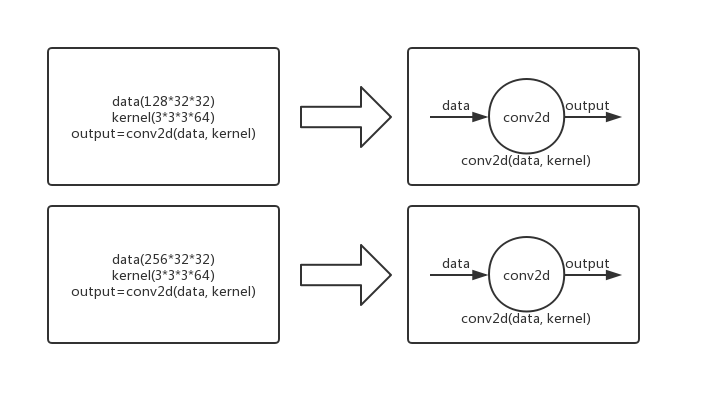
\includegraphics[width=0.8\textwidth]{figures/dag_same.jpg}
        \caption{图中预先定义的两个网络,输入的形状不同,但是生成的数据流图是相同的}
        \label{fig:dag_same}
    \end{figure}
    
\section{模型架构}    
    我们实现的预测模型整体架构如图\ref{fig:arch}所示。主要实现包含两部分,即图中的调度模拟,和性能模型两部分。其中,调度模拟部分根据深度神经网络应用在运行过程中生成的数据流图,模拟预测真实运行情况下每一个操作的运行状况,包括运行的顺序,运行所在设备,运行占用资源等。性能模型部分根据实际Tensorflow中操作运行的时间,建立操作性能模型。得到的结果再提供给调度模拟部分,两部分结合,继而在操作的粒度上,预测在正常的Tensorflow的调度下,深度神经网络应用的运行时间。
    
\subsection{调度模拟}
    Tensorflow中所有的计算任务会被转化为数据流图的形式,其中每个点代表一个计算操作,每一条边表示一组数据。具体到实际运行tensorflow中,每一个点代表一个计算函数,如矩阵乘法(MatMul),二维卷积(Conv2D)等。
    
    \begin{figure}[!htbp]
        \centering
        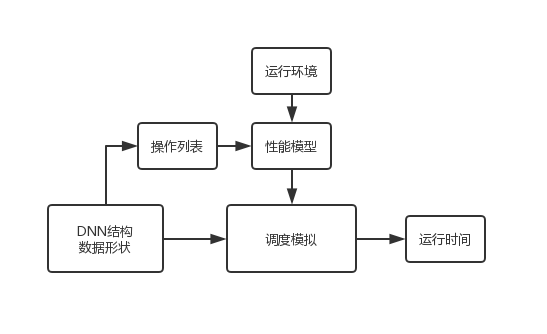
\includegraphics[width=0.8\textwidth]{figures/arch.jpg}
        \caption{预测模型整体架构}
        \label{fig:arch}
    \end{figure}

\subsection{调度预测}
    
    
\subsection{性能模型}